\section{Parte 2: Diagrama de Clases (UML)}

\subsection{Modelo del Dominio de SIGC-CUSCO}
El diagrama de clases modela la estructura estática del sistema, sus tipos de datos, operaciones y cardinalidades. El archivo nativo editable se ubica en \texttt{diagramas/diagrama\_clases\_sigc.drawio}.

\begin{figure}[H]
    \centering
    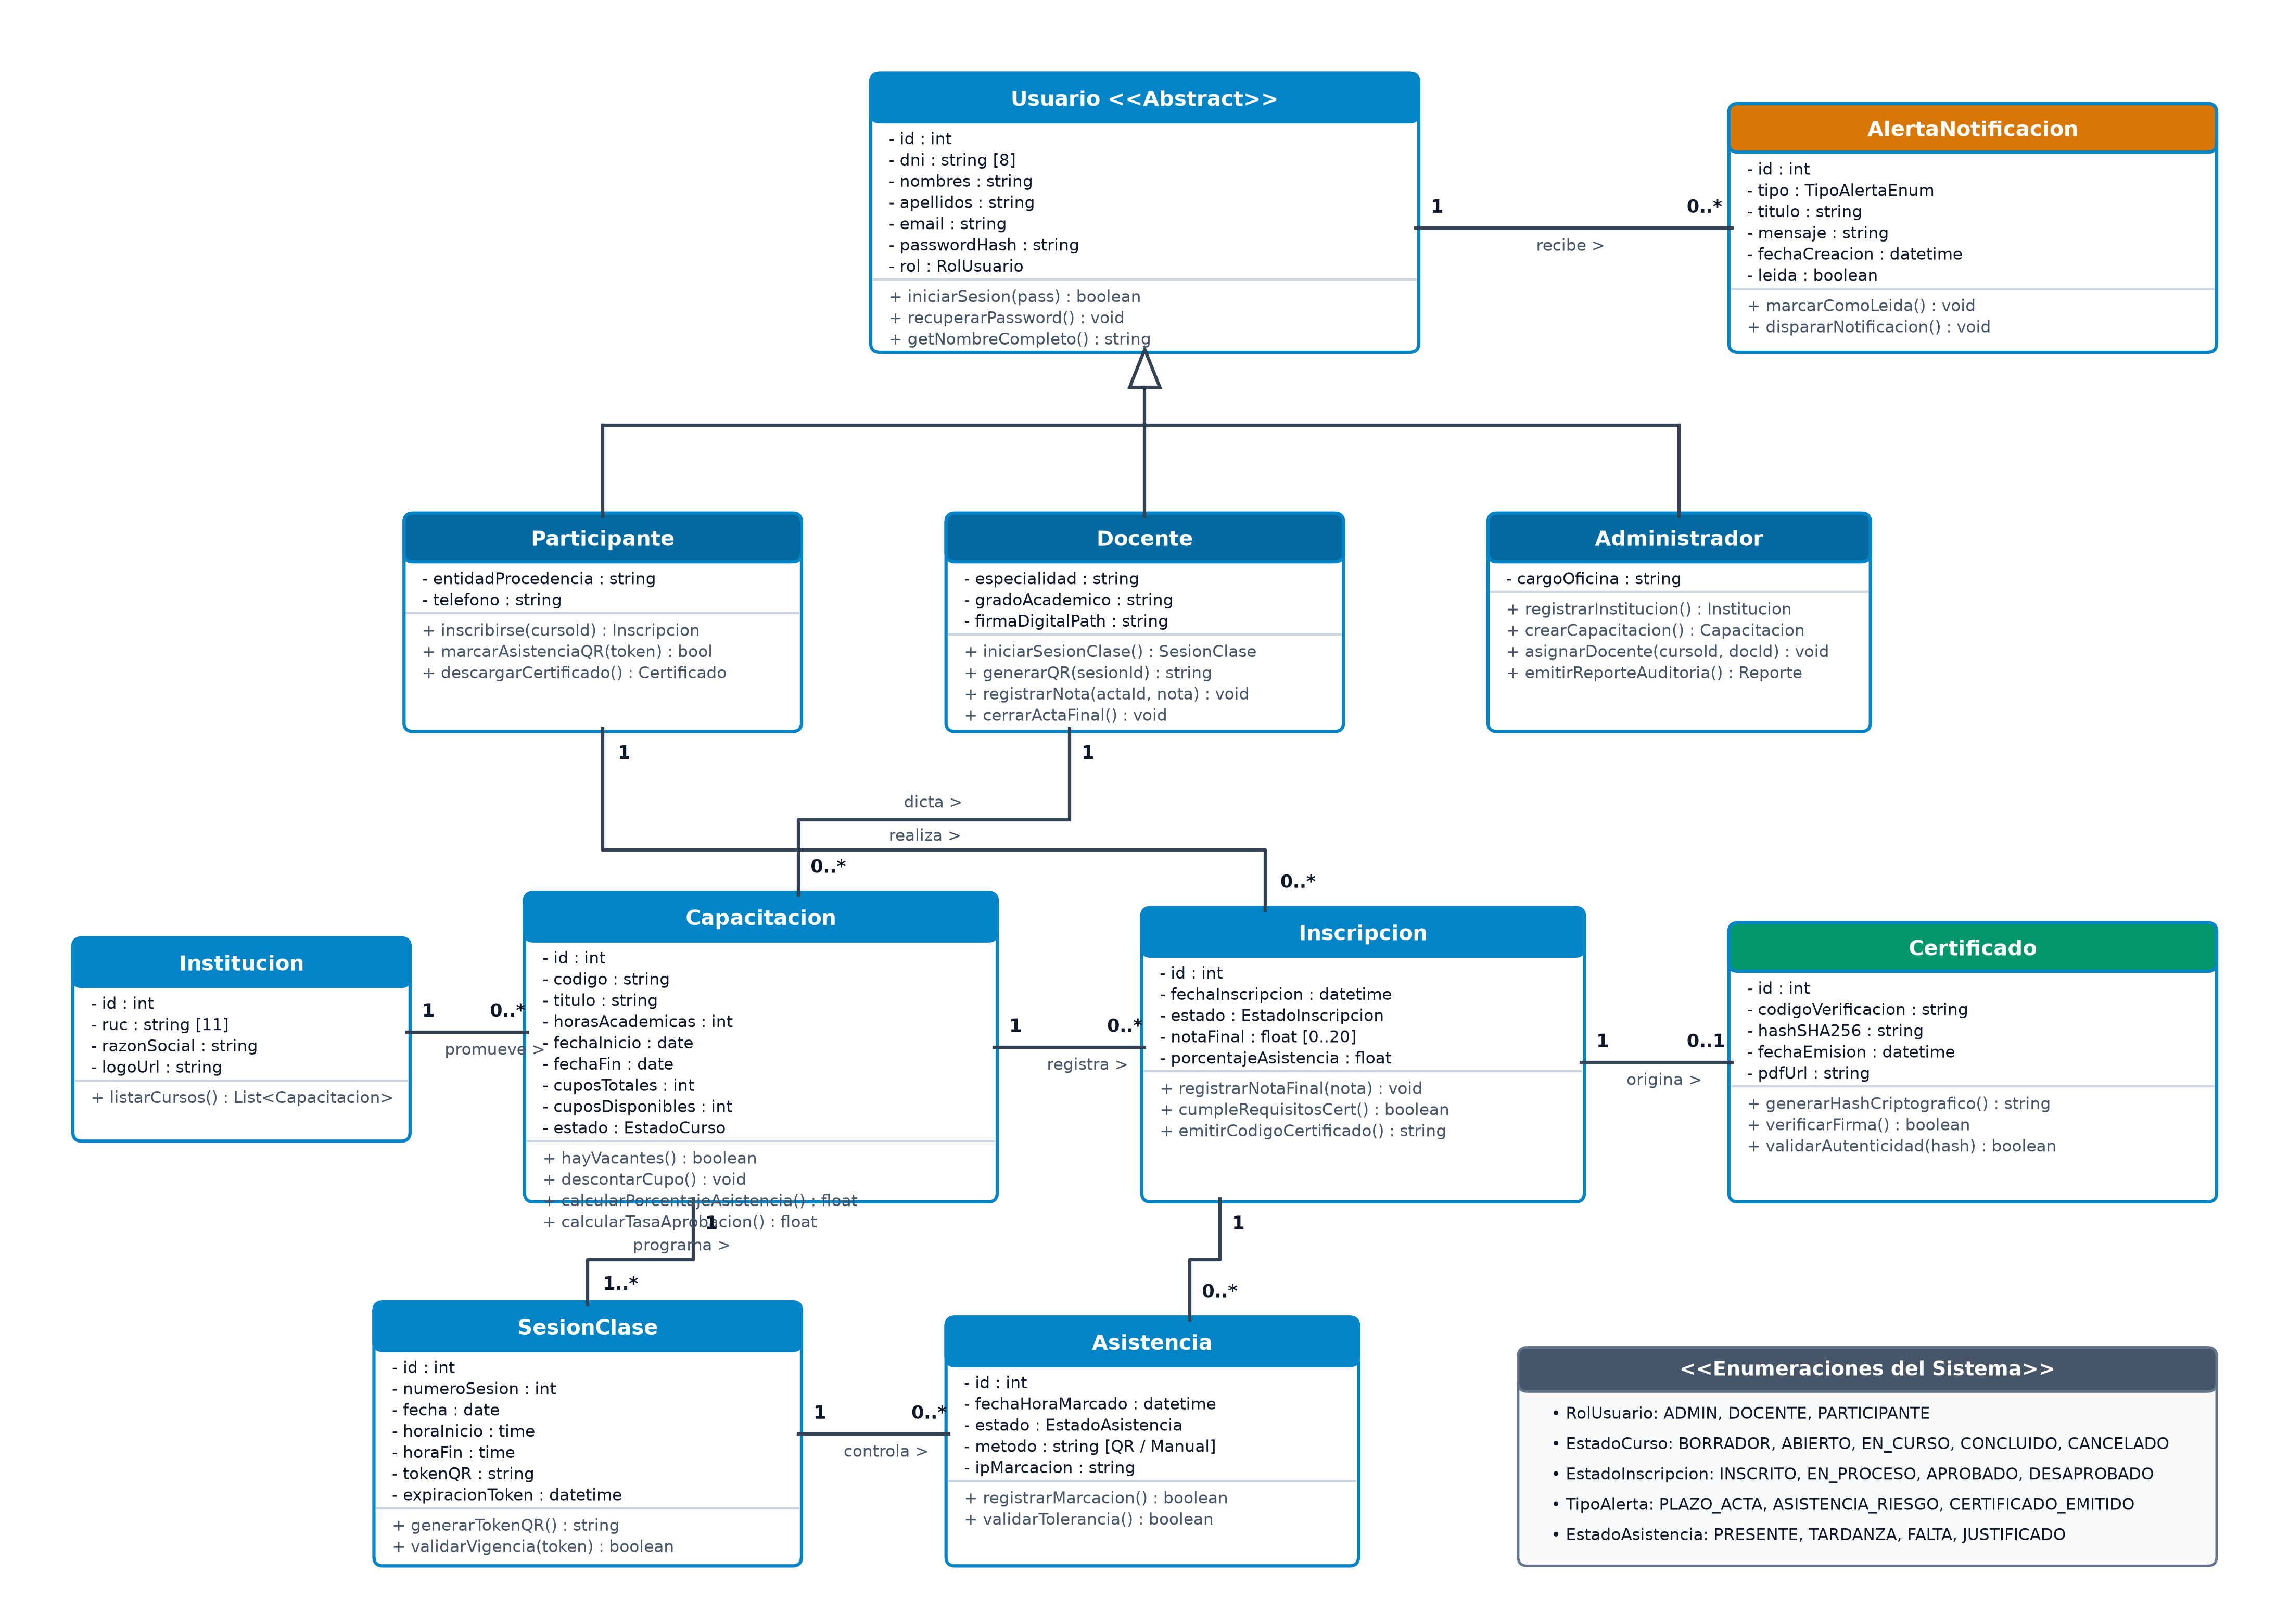
\includegraphics[width=0.98\textwidth]{diagrama_clases.png}
    \caption{Diagrama de Clases del Dominio de SIGC-CUSCO (Draw.io).}
    \label{fig:diagrama_clases}
\end{figure}

\begin{table}[H]
\centering
\footnotesize
\begin{tabularx}{\textwidth}{l l P{3.0cm} Y}
\toprule
\textbf{Clase Origen} & \textbf{Relación} & \textbf{Clase Destino} & \textbf{Semántica del Negocio} \\
\midrule
\texttt{Usuario} & Generalización & \texttt{Participante, Docente, Admin} & Herencia de credenciales (DNI, email, hash) y rol. \\
\texttt{Institucion} & $1 \longleftrightarrow 0..*$ & \texttt{Capacitacion} & Entidad que promueve cursos formativos. \\
\texttt{Docente} & $1 \longleftrightarrow 0..*$ & \texttt{Capacitacion} & Docente asignado a dictar la capacitación. \\
\texttt{Capacitacion} & $1 \longleftrightarrow 1..*$ & \texttt{SesionClase} & Un curso consta de una o más sesiones con código QR. \\
\texttt{Participante} & $1 \longleftrightarrow 0..*$ & \texttt{Inscripcion} & Ciudadano inscrito formalmente mediante su DNI. \\
\texttt{Capacitacion} & $1 \longleftrightarrow 0..*$ & \texttt{Inscripcion} & Control de vacantes y padrón nominal de matriculados. \\
\texttt{SesionClase} & $1 \longleftrightarrow 0..*$ & \texttt{Asistencia} & Registro de marcaciones de asistencia por sesión. \\
\texttt{Inscripcion} & $1 \longleftrightarrow 0..1$ & \texttt{Certificado} & Matrícula aprobada origina un certificado con hash SHA-256. \\
\texttt{Usuario} & $1 \longleftrightarrow 0..*$ & \texttt{AlertaNotificacion} & Envío de alertas de vencimiento de actas e inasistencias. \\
\bottomrule
\end{tabularx}
\caption{Relaciones y cardinalidades del Diagrama de Clases.}
\label{tab:relaciones_clases}
\end{table}
